\documentclass{article}

\usepackage{graphicx}
\usepackage{hyperref}
\usepackage{listings}
\usepackage{color}
\usepackage{lmodern}  % for bold teletype font
\usepackage{amsmath}  % for \hookrightarrow
\usepackage{xcolor}   % for \textcolor
\usepackage{biblatex}
\usepackage{soul}

 \lstnewenvironment{teX}[1][]
      {\lstset{language=[LaTeX]TeX}\lstset{escapeinside={(*@}{@*)},
       numbers=left,numberstyle=\normalsize,stepnumber=1,numbersep=5pt,
       breaklines=true,
       %firstnumber=last,
           %frame=tblr,
           framesep=5pt,
           basicstyle=\normalsize\ttfamily,
           showstringspaces=false,
           keywordstyle=\itshape\color{blue},
          %identifierstyle=\ttfamily,
           stringstyle=\color{maroon},
        commentstyle=\color{black},
        rulecolor=\color{black},
        xleftmargin=0pt,
        xrightmargin=0pt,
        aboveskip=\medskipamount,
        belowskip=\medskipamount,
               backgroundcolor=\color{white}, #1
    }}
    {}

\title{Evaluating Performance of Different FIFO Queues in the Java Virtual Machine's Garbage Collector}
\date{2019-03-16}
\author{Guy Ezer ; Ran Hochshtet}

% images path
\graphicspath { {./images/} }

% newline between paragraphs
\usepackage[parfill]{parskip}
\lstset{
  basicstyle=\ttfamily,
  columns=fullflexible,
  frame=single,
  breaklines=true,
  postbreak=\mbox{\textcolor{red}{$\hookrightarrow$}\space},
}

\begin{document}
  \maketitle

  \newpage

  \section{Intro}
  \subsection{Abstract}
  \paragraph
  Large-scale multicore architectures create new challenges for garbage collectors. 
  The paper \href{https://hal.inria.fr/hal-00868012/document}{``A study of the scalability of stop-the-world garbage collectors on multicores``} analyzed the HostSpot JVM`s garbage collector (GC) called \textbf{Parallel Scavenge}, identified its bottlenecks and tried to address them using parallel programming techniques - such as using a lock-free task queue - as we saw in class.

  The paper modified the HotSpot JVM to support the proposed changes and compared both the non-modified JVM and the modified JVM on standard benchmarks and showed that the lock-free approach improved the GC throughput.

 Further research can be done on the concurrent FIFO queue in the GC context - 
 the concurrent FIFO queue is a fundamental data structure, and designing efficient concurrent queues has attracted a lot of research attention.
 Today, the best performing queues still have contended hot spots (namely, the queue head and tail). These hot spots are particularly painful when queues are used on modern non-uniform memory access (NUMA) machines. These machines have multiple processors, each of which has multiple cores.
 The overhead of contended hot spots on a NUMA machine is very high because of the latency of transferring a cache line between processors is orders of magnitudes higher than transferring a line between cores in the same processor.

 In our work, focused on the parallel task queue and study the impact of using different concurrent queues as the GC scheduling queue on the GC itself and the application on NUMA systems.

 We developed our code on the a \href{https://github.com/guye1296/jvm-gc-fifo/}{following GitHub repository} (\href{https://github.com/guye1296/jvm-gc-fifo/invitations}{invite link}). The branch \textit{report} contains the most up-to-date code.

 During our work, we encountered a LOT of difficulties - mostly during the intergation of the queues into the JVM and during the initial compilation of the project.

 \subsection{Queues Tested}

 We used an existing queue project that was provided by Adam, which contains the implementation baseline lock-free queues: \textit{LCRQ\cite{lcrq}} and \textit{MS-QUEUE}\cite{msqueue}. With the addition of applying \textit{numa-transformations} over the synchronization variables of the queue - the \textit{head} and \textit{tail}.

 The idea in all transformations is to increase the amount of cache line transfers performed inside processors and decrease the amount performed between the processors.
 NUMA-transformations are heuristics for determining ownership over the synchronization variable - only the cores that are on the same processor as the owner can access the variable.

 The following NUMA-transformations are used: 

 \begin{itemize}
   \item \textbf{Simple Schedualing} - No estimation, wait for a pre-defined timeout, and when it expires compete for ownership.
   \item \textbf{Reference Counting} - A processor remains the owner as long as the number of cores that are in operation is greater than zero. In order to reduce contention, there is a flag per core
	 that marks if it is in a queue operation or not. The agent counts the number of flags
	 of the active node, when it falls to zero, it competes for ownership.
   \item \textbf{Cache Miss Sensing} - Periodically, the agent accesses the synchronization variable`s
	   cache line twice, the first time in order to retrieve the cache line and the second time
	   in order to check if the cache line is still owned by it (determined by measuring access
	   time). If the cache line is still owned by the sampling agent, it competes for ownership.
	   The main idea of this mechanism is that if the sampling processor took ownership of
	   the cache line and kept it, then there must be low contention on the variable at this
	   time.
   \item \textbf{Workload Adaptive Transformation} - Each core calculates
	   the moving average of the time between two consecutive operations (work time) and the
	   moving average of the time it was in operation (queue time). The queue time is determined
	   mainly by the time it takes the core to obtain ownership of the synchronization variable`s
	   cache line. These averages are used to estimate whether the processor should remain an
	   owner or not.
 \end{itemize}

 We will run benchmarks again MS-QUEUE and LCRQ with all of the four mentioned NUMA-transformations. In addition we will run benchmarks again the queues without any transformation and again the original implementation of the MS-QUEUE that was provided in the paper.

 \subsection{Parallel Scavenge}
 \textbf{Parallel Scavenge} is the default GC of OpenJDK`s HotSpot virtual machine and is the one that provides the best performance when the number of cores increases\cite{paper}
 Parallel Scalability is a stop-the-world GC, meaning that the GC pauses the application threads during collection to prevent concurrent memory accesses from the application.

 The garbage collection is activated once the the memory buffers that are provided to the application are full; The following diagram shows the phases of Parallel Scavenge:

 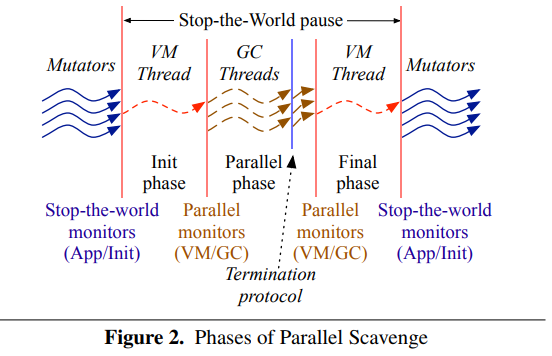
\includegraphics[width=\textwidth]{gc_phases.png}

 During the \textit{Initialisation Phase}, a single thread, called the VM thread, prepares GC tasks, which are executed in the \textit{Parallel Phase} by the GC threads.
 As soon as all the mutators are suspended, the VM thread initialises the queue of GC tasks. The task queue is implemented as a singly-linked list that is protected by a Monitor.

 Each GC thread fetches tasks from the queue in a concurrent matter. The \textit{Termination Protocol} is used to determine that the collection is done - meaning that every GC thread finished all its tasks and that there are no more GC tasks. 
 
 When the termination protocol finished - the \textit{Final Phase} begins. The \textit{Final Phase} mainly resizes the heap and wakes up the mutators.
 
 The paper showed an improvement in the GC throughput addressing the bottleneck caused by the queue's monitor - by changing the queue to a MS-QUEUE, which is \textbf{lock-free}, performance is improved due to threads not having to wait for the shared lock.

 \newpage

 \section{Integration}

 \subsection{Initial Compilation}
 We had \textit{a LOT} of problems during the compilation of the JVM.

 The Initial compilation of the provided version of OpenJDK took several days; We provide a script called \textit{compile.sh} which compiles the whole project.
 
 Since the code is very outdated, a lot of patches had to be made in order for the JDK to be compiled - which includes:
 \begin{itemize}
   \item Changing timestaps of older files - the build engine terminates when it encounters files that are over 10 years "old".
   \item Creating a local HTTP server to host resources that the build engine requires; the original server died:

   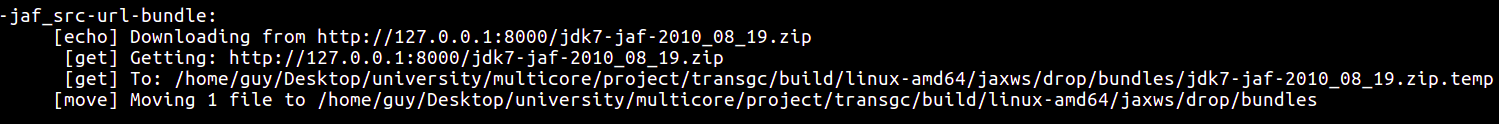
\includegraphics[width=\textwidth]{local_http_server.png}
   \item applying a few patches to libalsa (my distribution's libalsa was too new for the JDK to build on - the API was broken).
 \end{itemize}

 Luckily, we found the \href{http://www.voidcn.com/article/p-zayqisji-va.html}{following blog post} which covered the rest of the unresolved errors.

 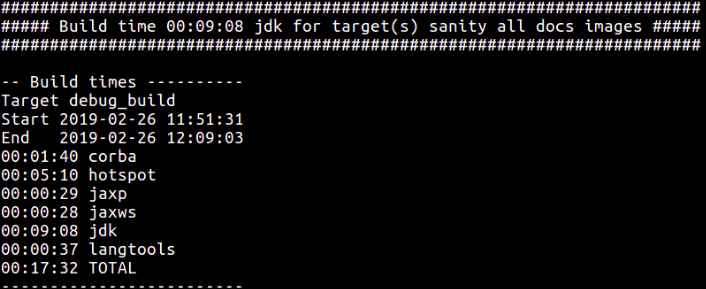
\includegraphics[width=\textwidth]{initial_build.png}

 \newpage

 \subsection{Integrating the NUMA Aware Queues} \label{queues:integration}
 After some thought, we decided that the queues that we want to integrate into the JVM will be linked against it as a \textbf{shared library}. Here are some supporting arguments:
 \begin{itemize}
   \item Hacking the build engine is complicated enough as is - many Makefile are generated and changes has to be made in several files, building as a shared library would probably take us less time.
   \item The queue library was compiled with specific flags and options; Applying the JVM`s build flags to the queue library could cause unexpected behavior or even fail the build.
   \item Compiling the JVM takes quite a while, and some times has to be compiled from scratch. Switching between NUMA transformation will only require to recompile the shared library and will result in shorter compilation times.
 \end{itemize}

 We maintain that library at \texttt{./msqueue-schedualing/}. 

 We then proceeded to define an API for the JVM to use:
 \begin{lstlisting}[language=C]
   extern void numa_enqueue(Globals* context, Object arg, int pid);

   extern Object numa_dequeue(Globals* context, int pid);
   
   extern Globals* create_global_context();
 \end{lstlisting}

 We tried to mask out the NUMA transformation method that is beging used and the queue structure from the JVM in order to create a consistant interface. Sadly, we have to re-compile the project when switching between MSQUEUE and LCRQ because the \textit{Globals} structure contains the inner queue definition.

 \begin{itemize}
   \item The \textit{Globals} is used to save the queue used and the schedualing method that was chosen.
   \item \textit{numa\_enqueue} is used to enqueue an address.
   \item \textit{numa\_dequeue} is used to dequeue an andress from the queue. If the queue is empty - it returns NULL.
 \end{itemize}

 Here is the implementation of the API. It can be seen that \textit{numa\_dequeue} performs a NUMA transformation on the queue's tail and head:

 \begin{lstlisting}[language=C]
   #include "numa_queue.h"
   
   extern void numa_enqueue(Globals* context, Object arg, int pid) {
       enqueue(&context->queue, arg, pid);
   }
   
   extern Object numa_dequeue(Globals* context, int pid){
       Object obj;
   
   #ifdef MSQUEUE
       cluster_scheduler_start_op(&context->atomic_scheduler, &context->queue.Head);
   #else
       cluster_scheduler_start_op(&context->atomic_scheduler, &context->queue.Head->head);
   #endif
       obj = (Object)(dequeue(&context->queue, pid));
   #ifdef MSQUEUE
       cluster_scheduler_end_op(&context->atomic_scheduler, &context->queue.Tail);
   #else
       cluster_scheduler_end_op(&context->atomic_scheduler, &context->queue.Tail->tail);
   #endif
       
       return obj;
   }
   
   extern Globals* create_global_context() {
       Globals* context = (Globals*)malloc(sizeof(Globals));
       SHARED_OBJECT_INIT(&context->queue);
   #ifdef MSQUEUE
       cluster_scheduler_init(&context->atomic_scheduler, &context->queue.Head, &context->queue.Tail);
   #else
       cluster_scheduler_init(&context->atomic_scheduler, &context->queue.Head->head, &context->queue.Tail->tail);
   #endif
       return context;
   }
 \end{lstlisting}

 For future reference, the following places in the JDK`s build system were changed in order to link agains \textit{libnuma\_queue}:
 \begin{itemize}
   \item \texttt{./hotspot/make/linux/build.sh} - Contains the top-level \textit{LD\_LIBRARY\_PATH}.

     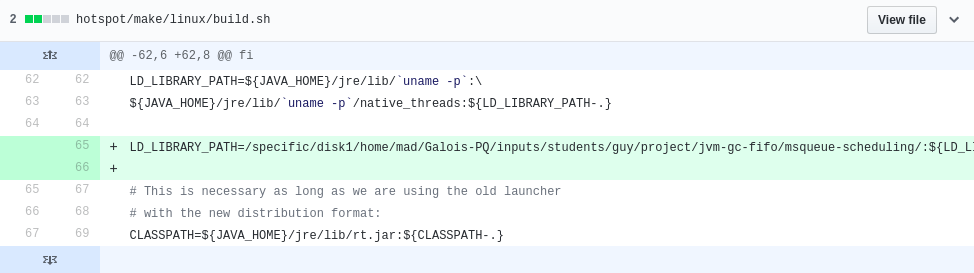
\includegraphics[width=\textwidth]{build.png}
   \item \texttt{./hotspot/make/linux/makefiles/buildtree.make} - Generator of Makefiles for different targets. Generated the Makefile for the Parallel Scavenge implementation.

     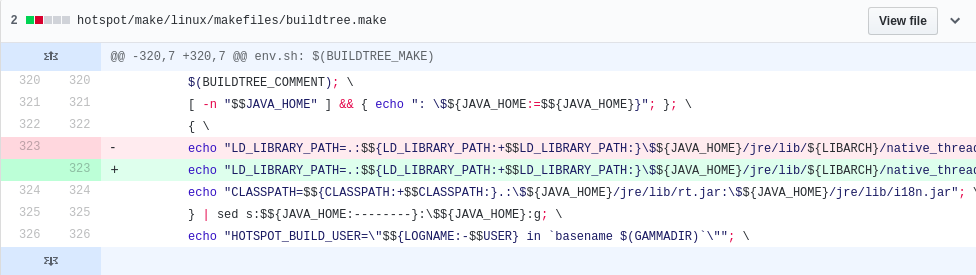
\includegraphics[width=\textwidth]{buildtree.png}
   \item \texttt{./hotspot/make/linux/makefiles/launcher.make} - Makefile for the gamma launcher, which is a required test that is run during the build (if we understood it correctly).

     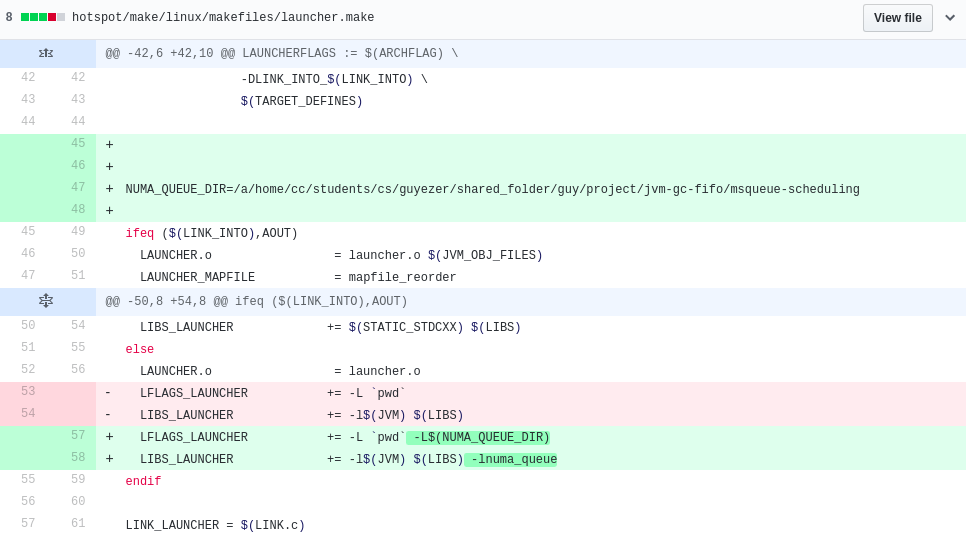
\includegraphics[width=\textwidth]{launcher.png}
 \end{itemize}

 \newpage

 \subsection{Replacing GC task queue with NUMA Aware Queues}
 The HotSpot JVM is a huge project with a lot of files and it was hard to find the exact location of the GC task queue.

 We found that the GC task queue is implemented in \textit{GCTaskQueue} located in \texttt{./hotspot/src/share/vm/gc\_implementation/parallelScavenge/gcTaskManager.hpp}.

 The methods we had to change were:
 \begin{lstlisting}[language=C]
  void initialize();
  virtual void destruct();
  void enqueue(GCTask* task);
  void enqueue(GCTaskQueue* list);
  GCTask* dequeue();
 \end{lstlisting}

 After we changed these methods and tested the JVM we noticed that the GC stuck after some minutes.
 We tried to understand why it's happening and we noticed that this happens when the GC-Manager call the \lstinline{enqueue(GCTaskQueue* list)}, and the list is not created on the heap. Thus we understood that we need to use the original queue in this case.
 Therefore we added two more methods:

 \begin{lstlisting}[language=C]
  void orig_enqueue(GCTask* task);
  GCTask* orig_dequeue();
 \end{lstlisting}

 The above methods are the methods of the original queue.

 Now we'll review the changes we inserted to the \textit{GCTaskQueue}:

 \begin{lstlisting}[language=C]
void GCTaskQueue::initialize() {
    if (!_is_c_heap_obj) {
        set_insert_end(NULL);
        set_remove_end(NULL);
        set_length(0);
    }
    else {
        if (context == NULL) {
            context = create_global_context();
        }
        set_length(0);
    }
}
 \end{lstlisting}

 In the \lstinline{initialize()} method we allocate memory for the NUMA-aware queue and initialize it. If the queue was allocated on the heap we use the original initialize steps.

 \begin{lstlisting}[language=C]
void GCTaskQueue::destruct() {
    free(context);
}
 \end{lstlisting}

 In the \lstinline{destruct()} method we free the memory we allocated for the NUMA-aware queue.

 \begin{lstlisting}[language=C]
void GCTaskQueue::enqueue(GCTask* task) {
    if (!_is_c_heap_obj) {
        orig_enqueue(task);
    }
    else {
        if (TraceGCTaskQueue) {
            tty->print_cr("[" INTPTR_FORMAT "]"
                    " GCTaskQueue::enqueue(task: "
                    INTPTR_FORMAT ")",
                    this, task);
            print("before:");
        }
        assert(task != NULL, "shouldn't have null task");
        numa_enqueue(context, (uint64_t)task, 0);
        increment_length();
        if (TraceGCTaskQueue) {
            print("after:");
        }
    }
}
 \end{lstlisting}

 In the \lstinline{enqueue(GCTask* task)} method if the queue was allocated on the heap, we enqueue the task to the NUMA-aware queue and increment the length of the queue by one. Otherwise we use the original enqueue method.

 \begin{lstlisting}[language=C]
void GCTaskQueue::enqueue(GCTaskQueue* list) {
  if (TraceGCTaskQueue) {
    tty->print_cr("[" INTPTR_FORMAT "]"
                  " GCTaskQueue::enqueue(list: "
                  INTPTR_FORMAT ")",
                  this);
    print("before:");
    list->print("list:");
  }
  if (list->is_empty()) {
    // Enqueuing the empty list: nothing to do.
    return;
  }

  uint list_length = list->length();
  GCTask* task;

  for (uint i = 0; i < list_length; ++i) {
      task = list->dequeue();
      enqueue(task);
  }

  set_length(length() + list_length);
  
  list->set_length(0);
  if (TraceGCTaskQueue) {
    print("after:");
    list->print("list:");
  }
}
 \end{lstlisting}

 In the \lstinline{enqueue(GCTaskQueue* list)} method we remove all the task from \lstinline{list} with the \lstinline{dequeue()} method, and insert all the tasks to the queue with the \lstinline{enqueue(GCTask* task)} method.

 \begin{lstlisting}[language=C]
GCTask* GCTaskQueue::dequeue() {
    if (!_is_c_heap_obj) {
        return orig_dequeue();
    }
    else {
        if (TraceGCTaskQueue) {
            tty->print_cr("[" INTPTR_FORMAT "]"
                    " GCTaskQueue::dequeue()", this);
            print("before:");
        }

        GCTask* result = (GCTask*)numa_dequeue(context, 0);
        if (result != NULL) {
            decrement_length();
        }

        if (TraceGCTaskQueue) {
            tty->print_cr("    return: " INTPTR_FORMAT, result);
            print("after:");
        }
        return result;
    }
}
 \end{lstlisting}

 In the \lstinline{dequeue()} method if the queue was allocated on the heap, we dequeue the task from the NUMA-aware queue and decrement the length of the queue by one. Otherwise we use the original dequeue method.

 We noticed that there is no need to change the method \lstinline{dequeue(uint affinity)} because the GC-Manager doesn't call that method in our case.

 \subsection{MS-QUEUE Bug Fix}

 When first running the MS-QUEUE implementation that was given in the repository a runtime error occured. After some debugging we figured out that there is a null pointer dereference in \texttt{./msqueue-schedualing/MSQUEUE/msqueue.c:enqueue}

 \begin{lstlisting}[language=C]
 void enqueue(queue_t* p_msqueu, Object arg, int pid) {
	node_t* node = new_node();	// Allocate a new node from the free list
	volatile node_t* tail = null;
	node_t* next = null;
	node->value = arg;	// Copy enqueued value into node
	node->next = null;	// Set next pointer of node to NULL
	reset_backoff(&backoff);
	while (true) {			// Keep trying until Enqueue is done
		//  *** null pointer dereference here ***
		tail = p_msqueu->Tail; 
		// Read Tail.ptr and Tail.count together
		next = tail->next;	
	...
 \end{lstlisting}

By using gdb watchpoints, We were able to find that the function that causes the dereference is \texttt{dequeue}:

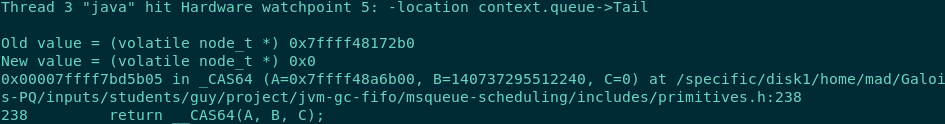
\includegraphics[width=\textwidth]{watchpoint.png}

Here, we can see that a CAS instruction caused NULL to be put in the queue's tail.
By applying backtrace, we found the \texttt{dequeue} causes the bug:

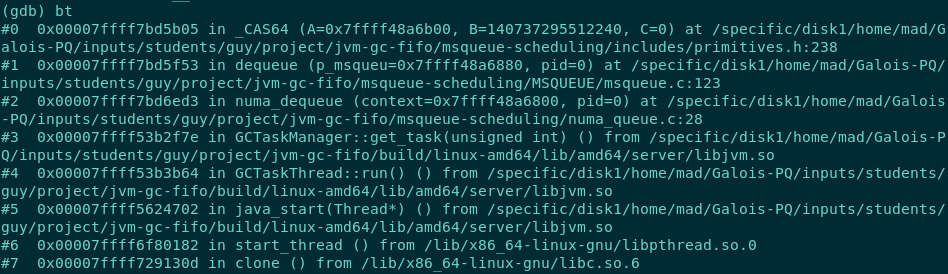
\includegraphics[width=\textwidth]{bt.png}

\texttt{dequeue}`s code:

\begin{lstlisting}[language=C]
Object dequeue(queue_t* p_msqueu, int pid) {
	volatile node_t *head, *tail, *next;
	Object value;

	// Keep trying until Dequeue is done
	while (true) { 
		head = p_msqueu->Head; 
		next = head->next;
		//Is queue empty
		if (next == NULL) { 
			tail = p_msqueu->Tail; 
			//If Tail is falling behind.  Try to advance it
			if (tail != next)
				CAS64(&p_msqueu->Tail, tail, next));
			else
				// Queue is empty, couldn't dequeue
				return NULL; 
			backoff_delay(&backoff);

		else {
			// No need to deal with Tail
			// Read value before CAS64
			// Otherwise, another dequeue might free the next node
			value = next->value;
			// Try to swing Head to the next node
			if (CAS64(&p_msqueu->Head, head, next)) {
			// Dequeue is done.  Exit loop
				break;
			}
			backoff_delay(&backoff);
		}
	}

	free_node(head);	// It is safe now to free the old node
	return value; // Queue was not empty, dequeue succeeded
}
	
\end{lstlisting}

If \texttt{dequeue} is applied to an empty queue, the following condition is correct:

\begin{lstlisting}[language=C]
if (tail != next)
    CAS64(&p_msqueu->Tail, tail, next));
\end{lstlisting}

This is true because \textit{tail} is not NULL but an actuall address, and \textit{next} is set to null because \textit{head} is an empty node. Here is the GDB output before the CAS:

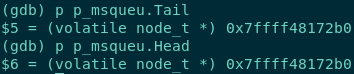
\includegraphics[width=\textwidth]{before-cas.png}

And here is the GDB output after the CAS:

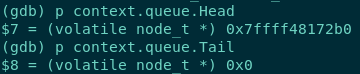
\includegraphics[width=\textwidth]{after-cas.png}

In our implementation, \lstinline{enqueue(GCTaskQueue* list)} calls \lstinline{dequeue} - meaning that a \lstinline{dequeue} is called before \lstinline{enqueue} - causing the said NULL pointer dereference.

The following changes were made to \texttt{dequeue} - note that we take advantage of that fact the \texttt{enqueue} and \texttt{dequeue} do not happen concurrently - because all of the \lstinline{enqueue} calls are called from the \textit{VM Thread} and are called before the \textit{Parallel Phase} \lstinline{dequeue}:

\begin{lstlisting}[language=C]
...
while (true) { // Keep trying until Dequeue is done
    head = p_msqueu->Head; 
    next = head->next; 

    if (p_msqueu->Head == p_msqueu->Tail) { 
        return NULL; 
...
\end{lstlisting}

\begin{itemize}
\item The condition check whether or not the queue is empty has changed to \texttt{p\_msqueu->Head == p\_msqueu->Tail} - because there are no enqueues this can be considered an atomic action, because tail is fixed.
\item The condition the check whether or not the tail has shifted is redundant because there are no enqueue calls - it is safe to return NULL.
\end{itemize}

 \newpage

 \section{Benchmarks}
 \subsection{Chosen Benchmarks}
 Initially, we wanted to run the same benchmarks that were introduced in the paper, but each came with its own set of problems:

 \begin{itemize}
   \item \textbf{SPECjbb2005} isn`t freely available.
   \item \textbf{DaCapo} was very unstable. We tried hacking it quite a bit but with not too much success.

	   We tried to ran \textit{tradesoap} and \textit{eclipse} and sometimes the run succeeded, and somtimes we ran into runtime errors:

 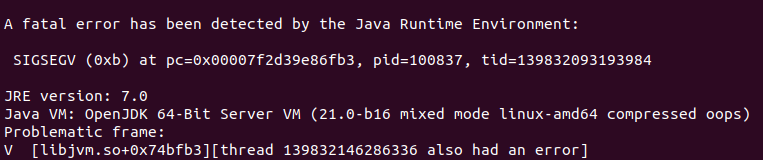
\includegraphics[width=\textwidth]{dacapo_error.png}

         This error occurred even when we used the java version that was installed on the server.
         After some research we found a post that suggest to avoid using parallelism options of the GC (the UseParallelOldGC option of the JVM). When we didn't use this option there were no runtime errors anymore.

         Thus, we decided to drop off this benchmark.
   \item \textbf{SPECjvm2008} - which several of its benchmarks were used in the paper. We only used \textit{transform.xml} because we did not have enough time to run all of the other benchmarks that were mentioned in the paper.
 \end{itemize}

 \subsection{Benchmarks Setup}
 We ran \textit{transform.xml} with an increasing number of cores dedicated for the GC.

 We set the heap size to 1GB, as specified in the paper.

 The GC's throughput is evaluated as:
 \begin{equation}
	 \frac{young\_generation\_work}{total\_time\_spent\_in\_\_young\_gc}
 \end{equation}

 \begin{itemize}
   \item \textit{young generation work} is the total bytes that were transferred in the young generation.
   \item \textit{total time spent in young gc} is the total execution time in young the GC generation.
 \end{itemize}

 Luckily for us, the initial author had already printed these values (and more) in the JVM exit point:

 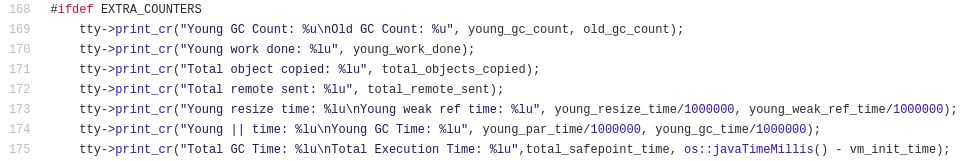
\includegraphics[width=\textwidth]{gc-debug-prints.png}

 The script \texttt{run\_benchmarks.sh} runs the benchmarks with different configurations - it iterates over all the different queues (msqueue and LCRQ), numa schedualing methods and an increasing number of cores. It saves the result to log files which are later on parsed by it into a .csv file - in which its left colomn is the number of processes and its right column is the GC throuhput for the given core.
This gave us the ability to quickly analyze results of different runs.

 \newpage

 \subsection{transform.xml Results}
 \subsubsection{Comparison of Different Queues}

 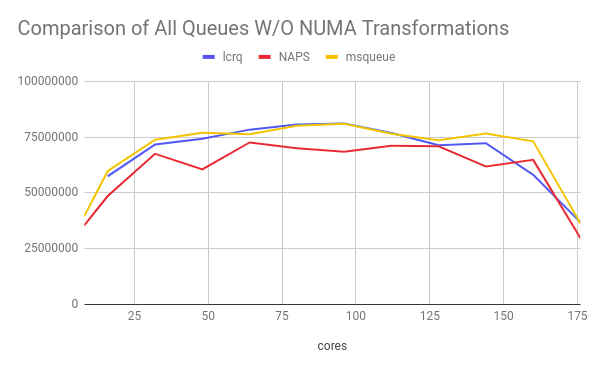
\includegraphics[width=\textwidth]{graph-no-schedule.png}

 It is seen that the original implementation (\textit{``NAPS``}) has the least amount of throughout (TP) between the three queues, and that given MSQUEUE and LCRQ have about the same performane - altough LCRQ has somewhat better performance in a high number of cores.

 ** TODO **

 \subsubsection{MSQUEUE}

 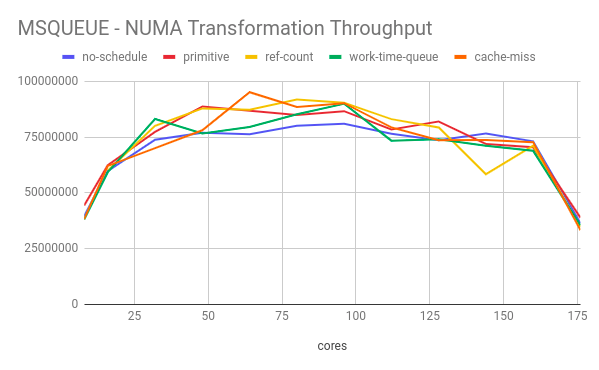
\includegraphics[width=\textwidth]{graph-msqueue.png}

 ** TODO **

 \subsubsection{LCRQ}

 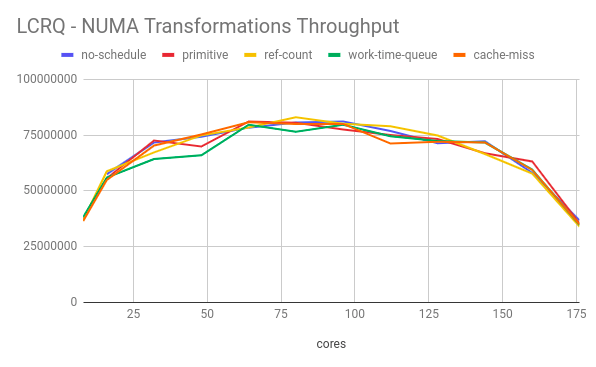
\includegraphics[width=\textwidth]{graph-lcrq.png}

 ** TODO **

 \subsection{Conclusion}

 ** TODO **

  % references
  \medskip
  \newpage

  \begin{thebibliography}{9}
    \bibitem{paper}
      Lokesh Gidra, Gael Thomas, Julien Sopena and Marc Shapiro: "A Study of the Scalability of Stop-the-world Garbage Collectors on Multicores"
      \\\texttt{https://hal.inria.fr/hal-00868012/document}
    \bibitem{lcrq}
      ``Fast Concurrent Queues for x86 Processors``
      \\\texttt{(https://www.cs.tau.ac.il/~mad/publications/ppopp2013-x86queues.pdf)}
    \bibitem{msqueue}
	    Maged M. Michael, Michael L. Scott: ``Simple, Fast, and Practical Non-Blocking and Blocking Concurrent Queue Algorithms``
      \\\texttt{http://www.cs.rochester.edu/~scott/papers/1996\_PODC\_queues.pdf}
  \end{thebibliography}

\end{document}
